\documentclass[a4paper,french]{article}

\usepackage[utf8]{inputenc}
\usepackage{ifpdf}

\ifpdf
\else
\usepackage[active]{srcltx}
\fi

\usepackage{amsmath}
\usepackage{amsfonts}
\usepackage{amssymb}

\usepackage[T1]{fontenc}
\usepackage{lmodern}

\usepackage{babel}
\usepackage{color}
\usepackage{graphicx}
\usepackage{mathrsfs}

\usepackage[np]{numprint}

\usepackage{hyperref}
\ifpdf
\hypersetup{pdftitle={Maillage vertical}, pdfauthor={Lionel Guez},
  hypertexnames=false, pdfstartview=FitBH}
\fi

                                %---------------

\newcommand{\ud}{\mathrm{d}}
\DeclareMathOperator{\tgh}{th}
\graphicspath{{Graphiques/}}

\author{Lionel GUEZ}
\title{Maillage vertical}

                                %---------------

\begin{document}

\maketitle
\tableofcontents
\listoffigures

\section[Coordonnée verticale hybride]{Définition de la
  coordonnée verticale hybride $\sigma$ -- pression}

Cf. \href{../../..//Documentation_LMDZ/Saint_Venant_LMDZ.pdf}{Intégration
  des équations de Saint-Venant avec LMDZ} et Eckermann (2009 882). On
pose :
\begin{equation}
  \begin{array}{|ll}
    b(0) = 0 \\
    b(s) = \exp(1 - 1 / s^2) & \mathrm{pour}\ s \in \mathbb{R}^*    
  \end{array}
  \label{eq:b}
\end{equation}
$b$ est $\mathscr{C}^\infty$ sur $\mathbb{R}$, paire, strictement croissante
sur $\mathbb{R}^+$. On a :
\begin{align*}
  & \exists \lim_{s \to +\infty} b(s) = e \\
  & b'(0) = 0 \\
  & b'(1) = 2
\end{align*}
et $b$ admet un point d'inflexion en $\sqrt{6} / 3$ ($\approx
\np{0,8}$). Cf. figure (\ref{fig:disvert}).
\begin{figure}[htbp]
  \centering
  %GNUPLOT: LaTeX picture with Postscript
\begin{picture}(0,0)%
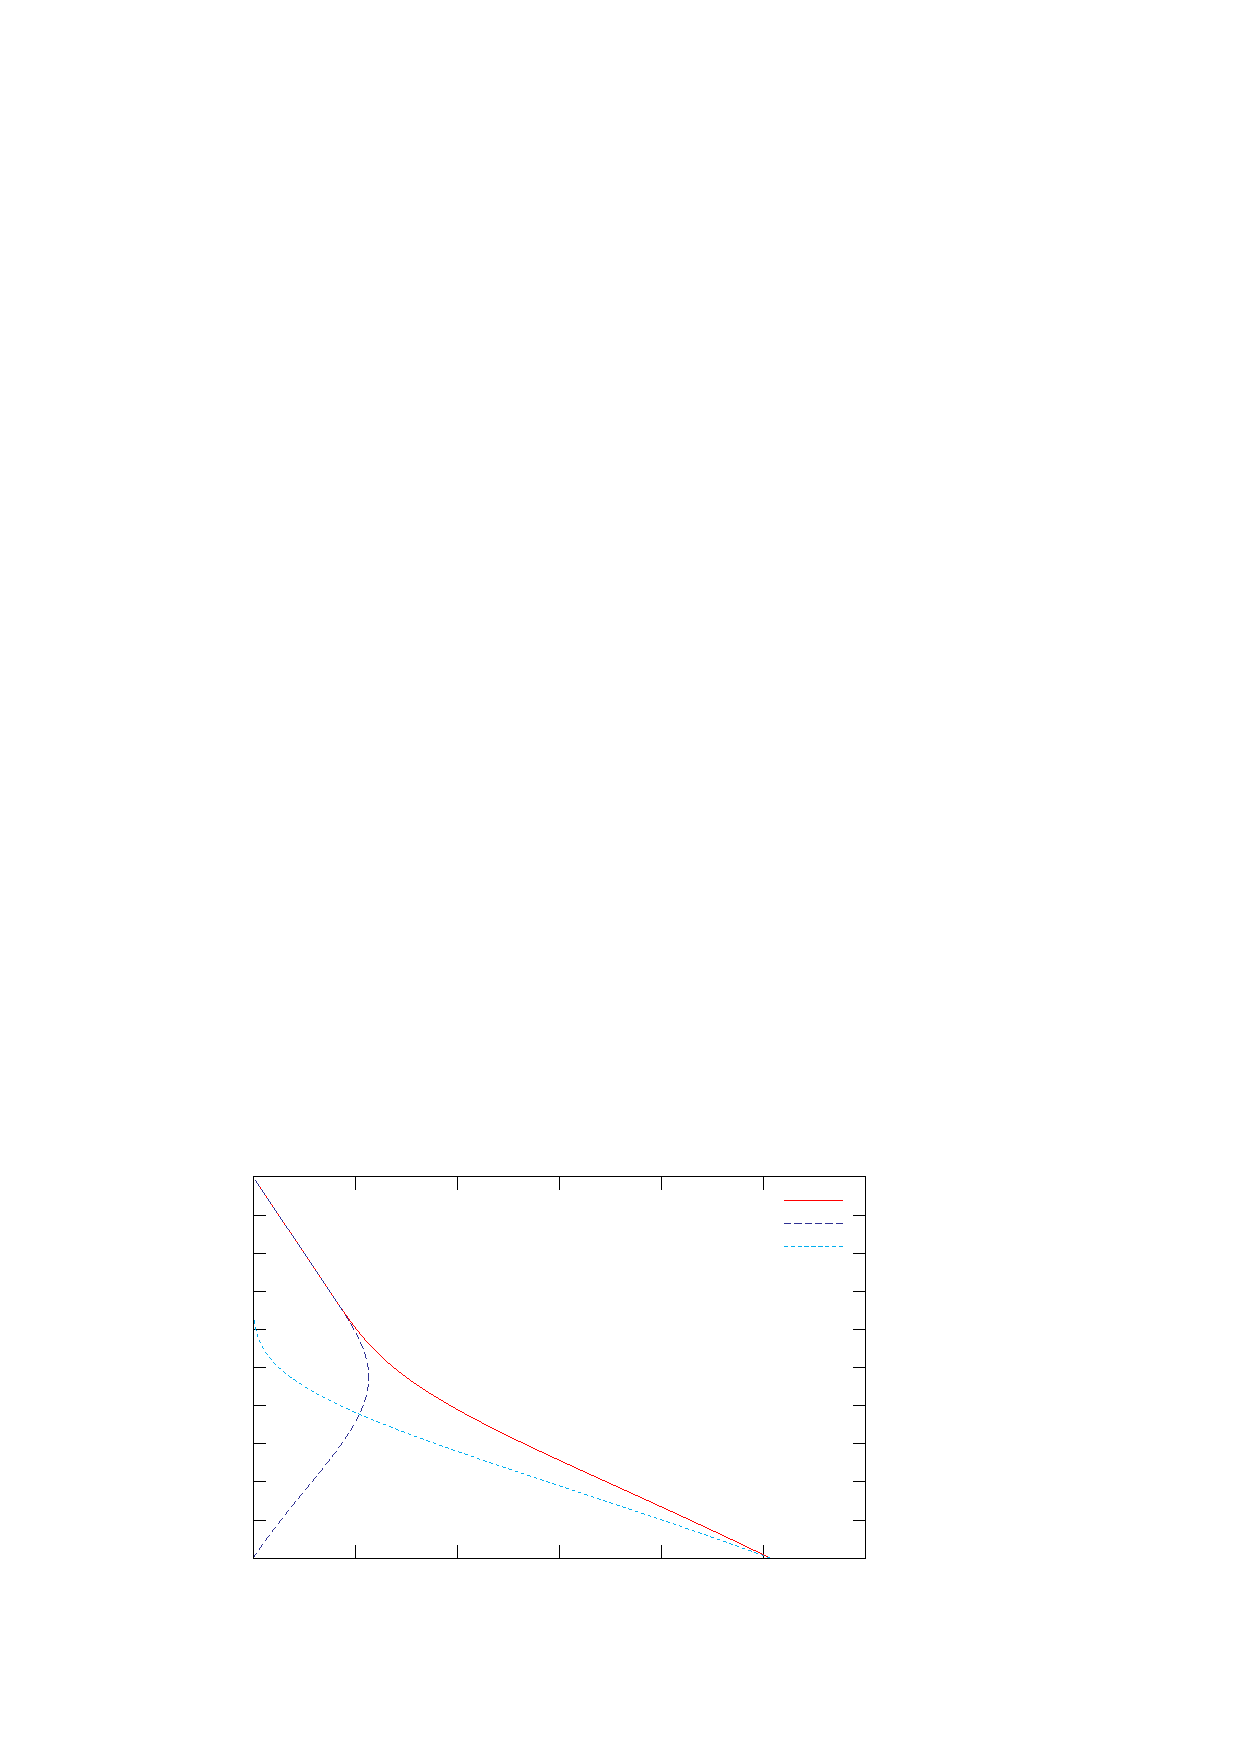
\includegraphics{Graphiques/disvert}%
\end{picture}%
\begingroup
\setlength{\unitlength}{0.0200bp}%
\begin{picture}(18000,10800)(0,0)%
\put(2200,10250){\makebox(0,0)[r]{\strut{} 0}}%
\put(2200,9335){\makebox(0,0)[r]{\strut{} 0.1}}%
\put(2200,8420){\makebox(0,0)[r]{\strut{} 0.2}}%
\put(2200,7505){\makebox(0,0)[r]{\strut{} 0.3}}%
\put(2200,6590){\makebox(0,0)[r]{\strut{} 0.4}}%
\put(2200,5675){\makebox(0,0)[r]{\strut{} 0.5}}%
\put(2200,4760){\makebox(0,0)[r]{\strut{} 0.6}}%
\put(2200,3845){\makebox(0,0)[r]{\strut{} 0.7}}%
\put(2200,2930){\makebox(0,0)[r]{\strut{} 0.8}}%
\put(2200,2015){\makebox(0,0)[r]{\strut{} 0.9}}%
\put(2200,1100){\makebox(0,0)[r]{\strut{} 1}}%
\put(2475,550){\makebox(0,0){\strut{} 0}}%
\put(4925,550){\makebox(0,0){\strut{} 20000}}%
\put(7375,550){\makebox(0,0){\strut{} 40000}}%
\put(9825,550){\makebox(0,0){\strut{} 60000}}%
\put(12275,550){\makebox(0,0){\strut{} 80000}}%
\put(14725,550){\makebox(0,0){\strut{} 100000}}%
\put(17175,550){\makebox(0,0){\strut{} 120000}}%
\put(550,5675){\rotatebox{90}{\makebox(0,0){\strut{}$s$}}}%
\put(14950,9675){\makebox(0,0)[r]{\strut{}$p$}}%
\put(14950,9125){\makebox(0,0)[r]{\strut{}$a$}}%
\put(14950,8575){\makebox(0,0)[r]{\strut{}$b \times p_s$}}%
\end{picture}%
\endgroup
\endinput

  \caption[Maillage vertical : $a$ et $b$]{Maillage vertical. Pour
    $p_a = 5 \cdot 10^4$ Pa et $p_s = \np{101325}$ Pa.}
  \label{fig:disvert}
\end{figure}
Puis, étant donné $p_a \in \mathbb{R}^{+*}$, on pose, pour tout
$s$ :
\begin{equation}
  a(s) = p_a (s - b(s))
  \label{eq:a}
\end{equation}
Pour $s > 0$ :
\begin{displaymath}
  a'(s) \ge 0 \Leftrightarrow b(s) \le s^3 / 2
\end{displaymath}
L'équation $b(s) = s^3 / 2$ admet deux solutions strictement
positives. Notons-les $s_1$ et $s_2$, $s_1 < 1 <
s_2$. ($s_1 \approx \np{0.53}, a(s_1) / p_a \approx \np{0.45}$.)
\begin{displaymath}
  \begin{array}{r|lcccccccr}
    s & 0 & & s_1 & & 1 & & s_2 & & + \infty \\
    \hline
    a(s) & & \nearrow & & \multicolumn{3}{c}{\searrow} & & \nearrow
    & \\
    \hline
  \end{array}
\end{displaymath}
$a$ est strictement croissante sur $[0, s_1]$,
strictement décroissante sur $[s_1, s_2]$, strictement
croissante sur $[s_2, + \infty[$. Cf. figure (\ref{fig:disvert}).
Enfin, étant donné $p_s \in \mathbb{R}^{+*}$, on pose, pour tout
$s$ :
\begin{align*}
  p(s) & = a(s) + b(s) p_s \\
  & = p_a s + b(s) (p_s - p_a)
\end{align*}
Cf. figure (\ref{fig:disvert}). On a :
\begin{displaymath}
  p(s) \underset{s \to 0}{\sim} p_a s
\end{displaymath}
Pratiquement :
\begin{displaymath}
  s \le \np{0,3} \Rightarrow b(s) \ll s
\end{displaymath}
Cf. figure (\ref{fig:b_s}).
\begin{figure}[htbp]
  \centering
  %GNUPLOT: LaTeX picture with Postscript
\begin{picture}(0,0)%
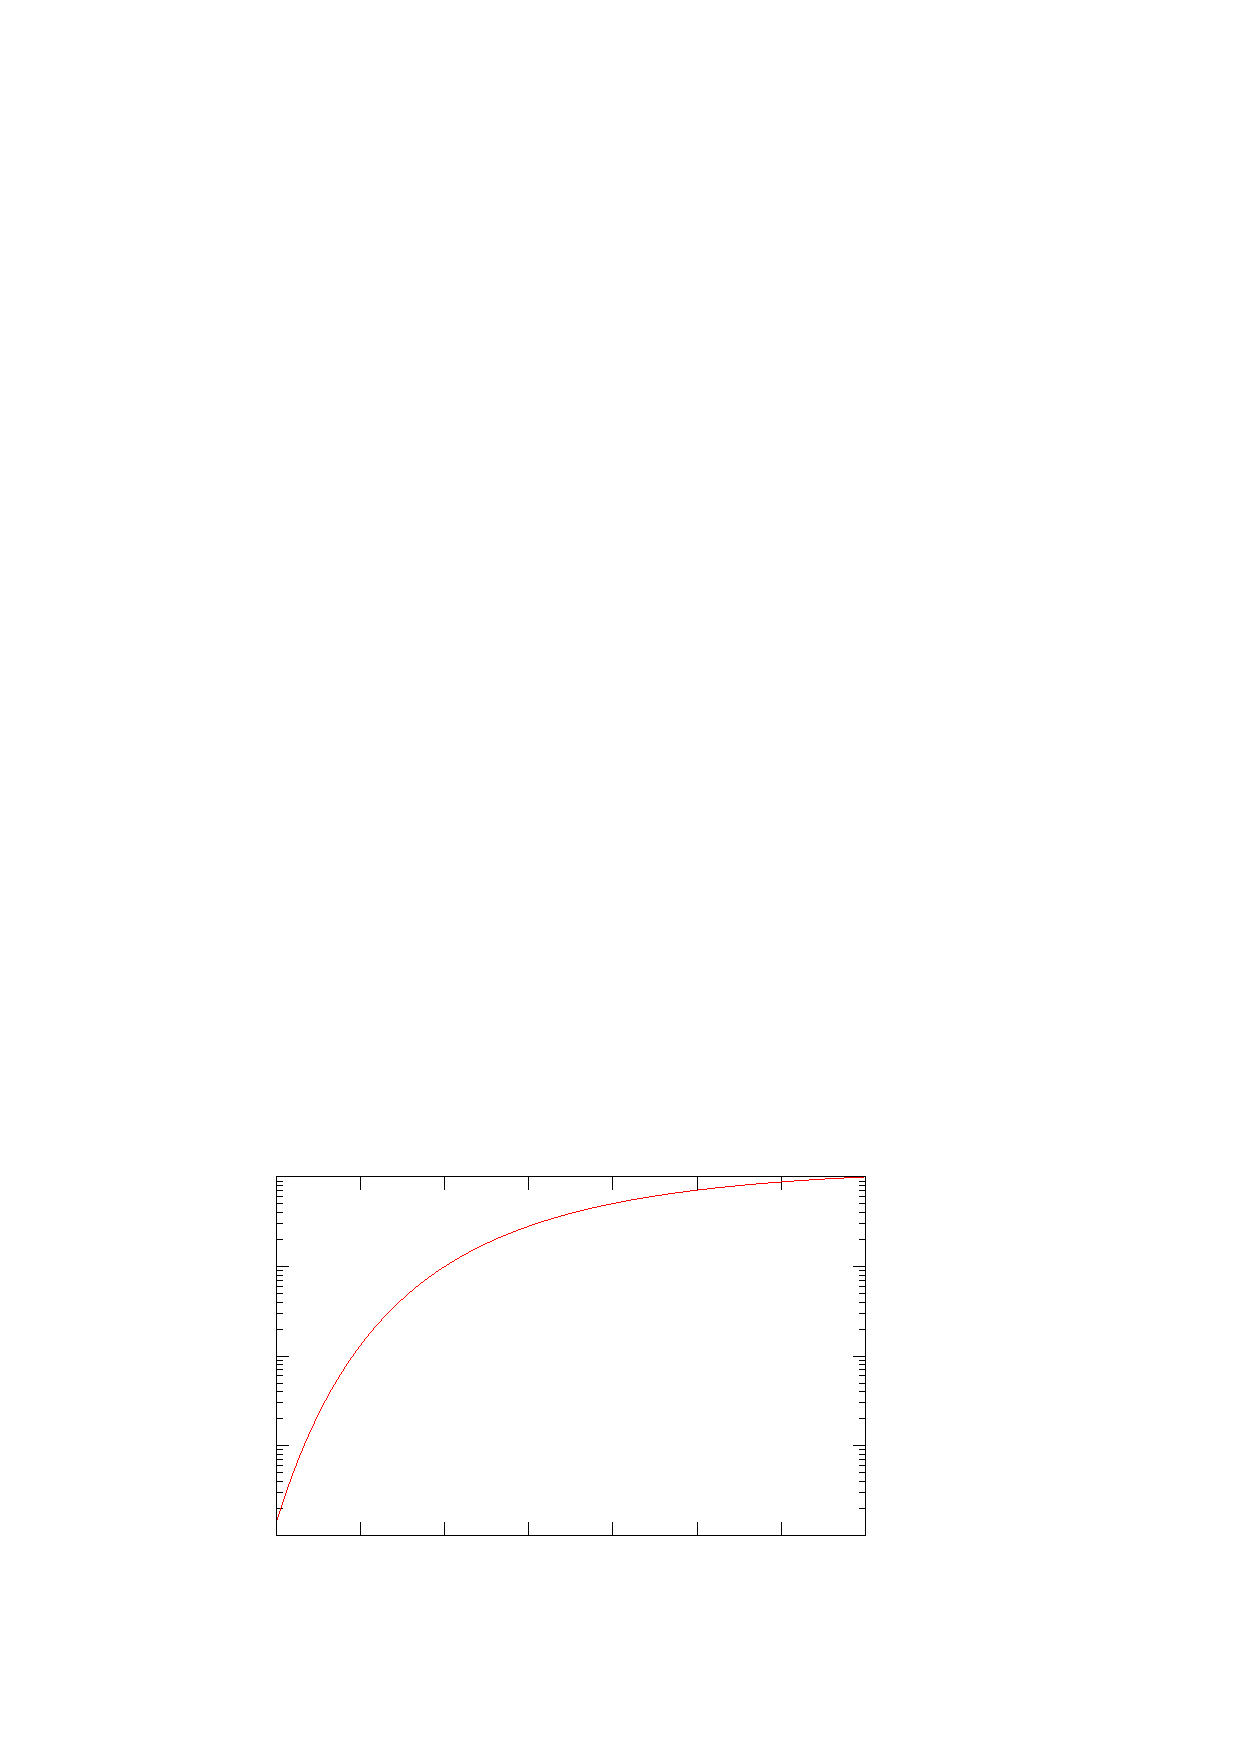
\includegraphics{Graphiques/b_s}%
\end{picture}%
\begingroup
\setlength{\unitlength}{0.0200bp}%
\begin{picture}(18000,10800)(0,0)%
\put(2750,1650){\makebox(0,0)[r]{\strut{} 1e-04}}%
\put(2750,3800){\makebox(0,0)[r]{\strut{} 0.001}}%
\put(2750,5950){\makebox(0,0)[r]{\strut{} 0.01}}%
\put(2750,8100){\makebox(0,0)[r]{\strut{} 0.1}}%
\put(2750,10250){\makebox(0,0)[r]{\strut{} 1}}%
\put(3025,1100){\makebox(0,0){\strut{} 0.3}}%
\put(5046,1100){\makebox(0,0){\strut{} 0.4}}%
\put(7068,1100){\makebox(0,0){\strut{} 0.5}}%
\put(9089,1100){\makebox(0,0){\strut{} 0.6}}%
\put(11111,1100){\makebox(0,0){\strut{} 0.7}}%
\put(13132,1100){\makebox(0,0){\strut{} 0.8}}%
\put(15154,1100){\makebox(0,0){\strut{} 0.9}}%
\put(17175,1100){\makebox(0,0){\strut{} 1}}%
\put(550,5950){\rotatebox{90}{\makebox(0,0){\strut{}$\frac{b(s)}{s}$}}}%
\put(10100,275){\makebox(0,0){\strut{}$s$}}%
\end{picture}%
\endgroup
\endinput

  \caption[Maillage vertical : $b(s) / s$]{Maillage vertical. Les
    niveaux de $s$ sont des niveaux de pression lorsque $b(s) / s$ est
    très petit.}
  \label{fig:b_s}
\end{figure}
En supposant :
\begin{equation*}
  |p_s - p_a| \lesssim p_a  
\end{equation*}
on a donc, aux plus hauts niveaux de l'atmosphère, tels que $s_l \le
\np{0,3}$ :
\begin{displaymath}
  p(s_l) \approx a(s_l)
  \approx p_a s_l
\end{displaymath}
En haut de l'atmosphère, les niveaux de $s$ sont des niveaux de
pression. Ces niveaux de pression sont les valeurs de \verb+ap+.
(Après une exécution de \verb+ce0l+, \verb+ap+ est dans le
fichier \verb+start.nc+.)

Numériquement, pour $s$ petit, il n'est pas possible de récupérer $s$
à partir de $b$ seulement. Mais, pour toute valeur de $s$, nous pouvons
récupérer $s$ à partir de $a$ et $b$ :
\begin{displaymath}
  s = a / p_a + b
\end{displaymath}

On a, pour $s$ non nul :
\begin{displaymath}
  p'(s) = p_a + 2 (p_s - p_a) b(s) / s^3
\end{displaymath}
Si $p_s \ge p_a$ alors $p'(s) > 0$ sur $\mathbb{R}^{+*}$ et $p(s)$ est
strictement croissante sur $\mathbb{R}^+$. De plus :
\begin{displaymath}
    p'(s) \underset{s \to 0}{\sim} p_a
\end{displaymath}
Pour $p_s = p_\mathrm{ref} > p_a$, le tableau $p(s_l)$ est
strictement décroissant de $p(1) = p_\mathrm{ref}$ à $p(0) = 0$. Donc
le tableau \verb+presnivs+ est strictement décroissant d'une valeur
strictement inférieure à $p_\mathrm{ref}$ à une valeur strictement
positive.

En utilisant une hauteur d'échelle $H = 7$ km constante, on définit
l'altitude-pression correspondant à $s$ :
\begin{displaymath}
  z(s) = H \ln \frac{p_s}{p(s)}
\end{displaymath}
Alors :
\begin{align*}
  & z(s=1) = 0 \\
  & z(s) \underset{s \to 0}{\sim} - H \ln s \\
  & z'(s) \underset{s \to 0}{\sim} - H / s
\end{align*}
En dehors du voisinage de 0, $z'(s)$ n'est pas monotone. Cf. figure
(\ref{fig:dz_ds}).
\begin{figure}[htbp]
  \centering
  \input{Graphiques/dz_ds.tex}
  \caption[Maillage vertical : $z'(s)$]{Maillage vertical. $z'(s)$ pour
    $p_a = 5 \cdot 10^4$ Pa, $p_s = \np{101325}$ Pa et $H = 7$
    km.}
  \label{fig:dz_ds}
\end{figure}

Quelle est la base naturelle associée aux coordonnées curvilignes
$(\lambda, \phi, s)$ ? On a :
\begin{equation*}
  (\partial_\lambda z)_s
  = (\partial_\lambda z)_p + (\partial_p z) (\partial_\lambda p)_s
\end{equation*}
et :
\begin{equation*}
  (\partial_\lambda p)_s = b \partial_\lambda p_s
\end{equation*}
Idem pour les dérivées partielles par rapport à $\phi$. Par ailleurs :
\begin{equation*}
  \partial_s z = (\partial_p z) \partial_s p
\end{equation*}
et :
\begin{equation*}
  \partial_s p = \frac{\ud a}{\ud s} + p_s \frac{\ud b}{\ud s}
\end{equation*}
D'où :
\begin{align*}
  & \mathbf{e}_\lambda
  = \mathscr{R} \mathbf{i}
    +
    \left[
    (\partial_\lambda z)_p - \frac{b}{\rho g} \partial_\lambda p_s
    \right]
    \mathbf{k} \\
  & \mathbf{e}_\phi
    =  r \mathbf{j}
    +
    \left[
    (\partial_\phi z)_p - \frac{b}{\rho g} \partial_\phi p_s
    \right]
    \mathbf{k} \\
  & \mathbf{e}_s
    = - \frac{1}{\rho g}
    \left(\frac{\ud a}{\ud s} + p_s \frac{\ud b}{\ud s} \right) \mathbf{k}
\end{align*}
La base duale est :
\begin{align*}
  & \mathbf{e}^\lambda = \frac{1}{\mathscr{R}} \mathbf{i} \\
  & \mathbf{e}^\phi = \frac{1}{r} \mathbf{j} \\
  & \mathbf{e}^s = \nabla s
\end{align*}
Cf. \href{../../../../Apprentissage/Dynamic_meteorology_texfol/dynamic_meteorology.pdf}{Météorologie
  dynamique}. Or :
\begin{equation*}
  \nabla p = \nabla a + b \nabla p_s + p_s \nabla b
\end{equation*}
donc :
\begin{equation*}
  \rho [(\nabla \Phi)_p - g \mathbf{k}]
  = \left(\frac{\ud a}{\ud s} + p_s \frac{\ud b}{\ud s} \right) \nabla s
  + b \nabla p_s
\end{equation*}
donc :
\begin{equation*}
  \mathbf{e}^s
  = \frac{1}{\frac{\ud a}{\ud s} + p_s \frac{\ud b}{\ud s}}
  [\rho (\nabla \Phi)_p - \rho g \mathbf{k} - b \nabla p_s]
\end{equation*}

\section{Discrétisation}

L'indice de niveau vertical est croissant de la surface au sommet de
l'atmosphère.  Cf. figure (\ref{fig:vertical_s}).
\begin{figure}[htbp]
  \centering
  \includegraphics[width=\textwidth]{vertical_s}
  \caption{Discrétisation du maillage vertical.}
  \label{fig:vertical_s}
\end{figure}

Dans \verb+disvert+, $s$ peut être calculé de trois façons selon la
valeur de \verb+vert_sampling+. Les trois échantillonnages de $s$ sont
comparés pour quelques valeurs de \verb+llm+ dans les figures
(\ref{fig:compare_sampl_9}), (\ref{fig:compare_sampl_19}),
(\ref{fig:compare_sampl_30}) et (\ref{fig:compare_sampl_41}).
\begin{figure}[htbp]
  \centering
  %GNUPLOT: LaTeX picture with Postscript
\begin{picture}(0,0)%
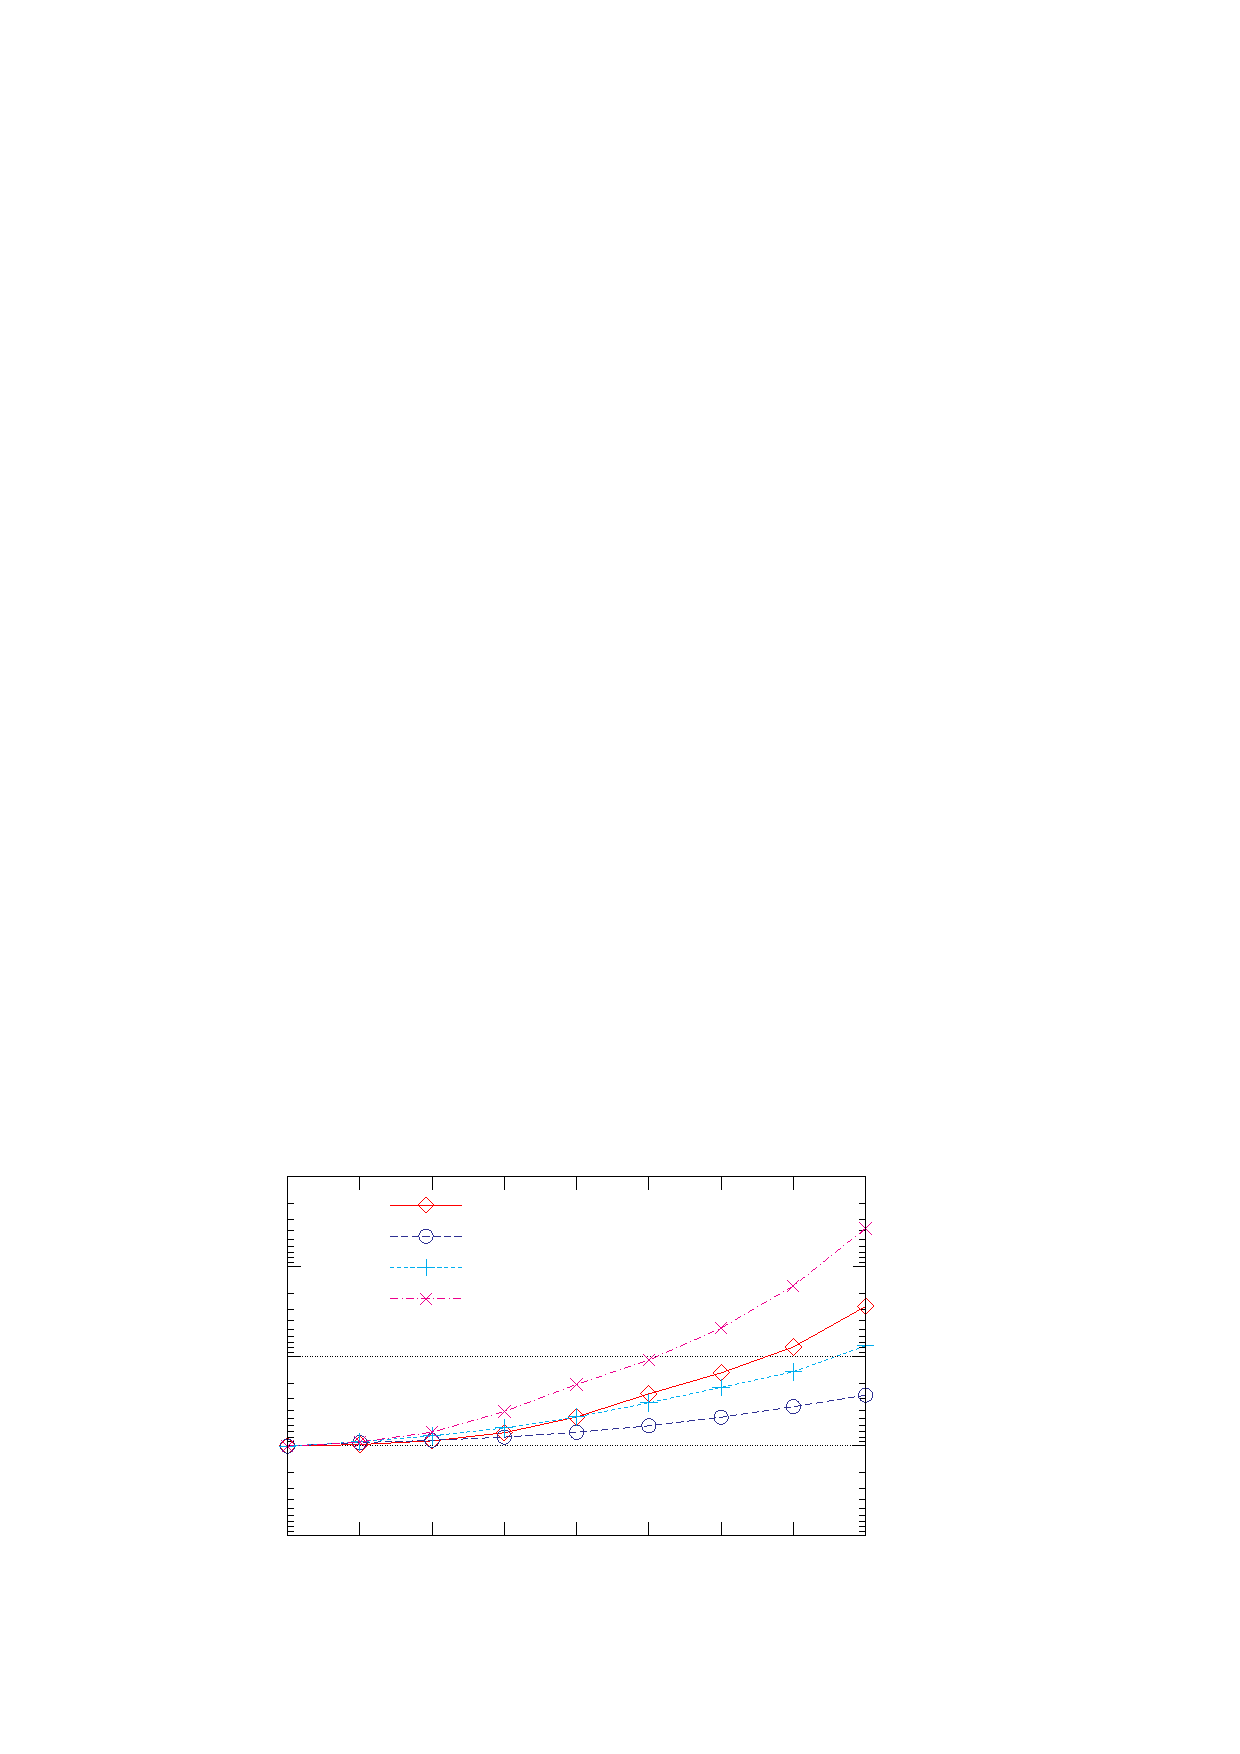
\includegraphics{Graphiques/compare_sampl_9}%
\end{picture}%
\begingroup
\setlength{\unitlength}{0.0200bp}%
\begin{picture}(18000,10800)(0,0)%
\put(3025,10250){\makebox(0,0)[r]{\strut{} 100}}%
\put(3025,8100){\makebox(0,0)[r]{\strut{} 1000}}%
\put(3025,5950){\makebox(0,0)[r]{\strut{} 10000}}%
\put(3025,3800){\makebox(0,0)[r]{\strut{} 100000}}%
\put(3025,1650){\makebox(0,0)[r]{\strut{} 1e+06}}%
\put(3300,1100){\makebox(0,0){\strut{} 1}}%
\put(5034,1100){\makebox(0,0){\strut{} 2}}%
\put(6769,1100){\makebox(0,0){\strut{} 3}}%
\put(8503,1100){\makebox(0,0){\strut{} 4}}%
\put(10238,1100){\makebox(0,0){\strut{} 5}}%
\put(11972,1100){\makebox(0,0){\strut{} 6}}%
\put(13706,1100){\makebox(0,0){\strut{} 7}}%
\put(15441,1100){\makebox(0,0){\strut{} 8}}%
\put(17175,1100){\makebox(0,0){\strut{} 9}}%
\put(550,5950){\rotatebox{90}{\makebox(0,0){\strut{}\shortstack{pression
        \\ (Pa)}}}}%
\put(10237,275){\makebox(0,0){\strut{}indice}}%
\put(5500,9575){\makebox(0,0)[r]{\strut{}LMD5}}%
\put(5500,8825){\makebox(0,0)[r]{\strut{}param}}%
\put(5500,8075){\makebox(0,0)[r]{\strut{}strato1}}%
\put(5500,7325){\makebox(0,0)[r]{\strut{}strato2}}%
\end{picture}%
\endgroup
\endinput

  \caption[Maillage vertical, échantillonnages de $s$ pour :
  \texttt{llm} = 9]{Maillage vertical.  Comparaison des trois
    échantillonnages de $s$ pour : \texttt{llm} = 9 ; \texttt{h} = 7 ;
    \texttt{deltaz} = \np{0,04} ; \texttt{beta} = \np{1,3} ;
    \texttt{k0} = 20 ; \texttt{k1} = \np{1,2}. La pression à la
    surface choisie est de 101325 Pa.}
  \label{fig:compare_sampl_9}
\end{figure}
\begin{figure}[htbp]
  \centering
  %GNUPLOT: LaTeX picture with Postscript
\begin{picture}(0,0)%
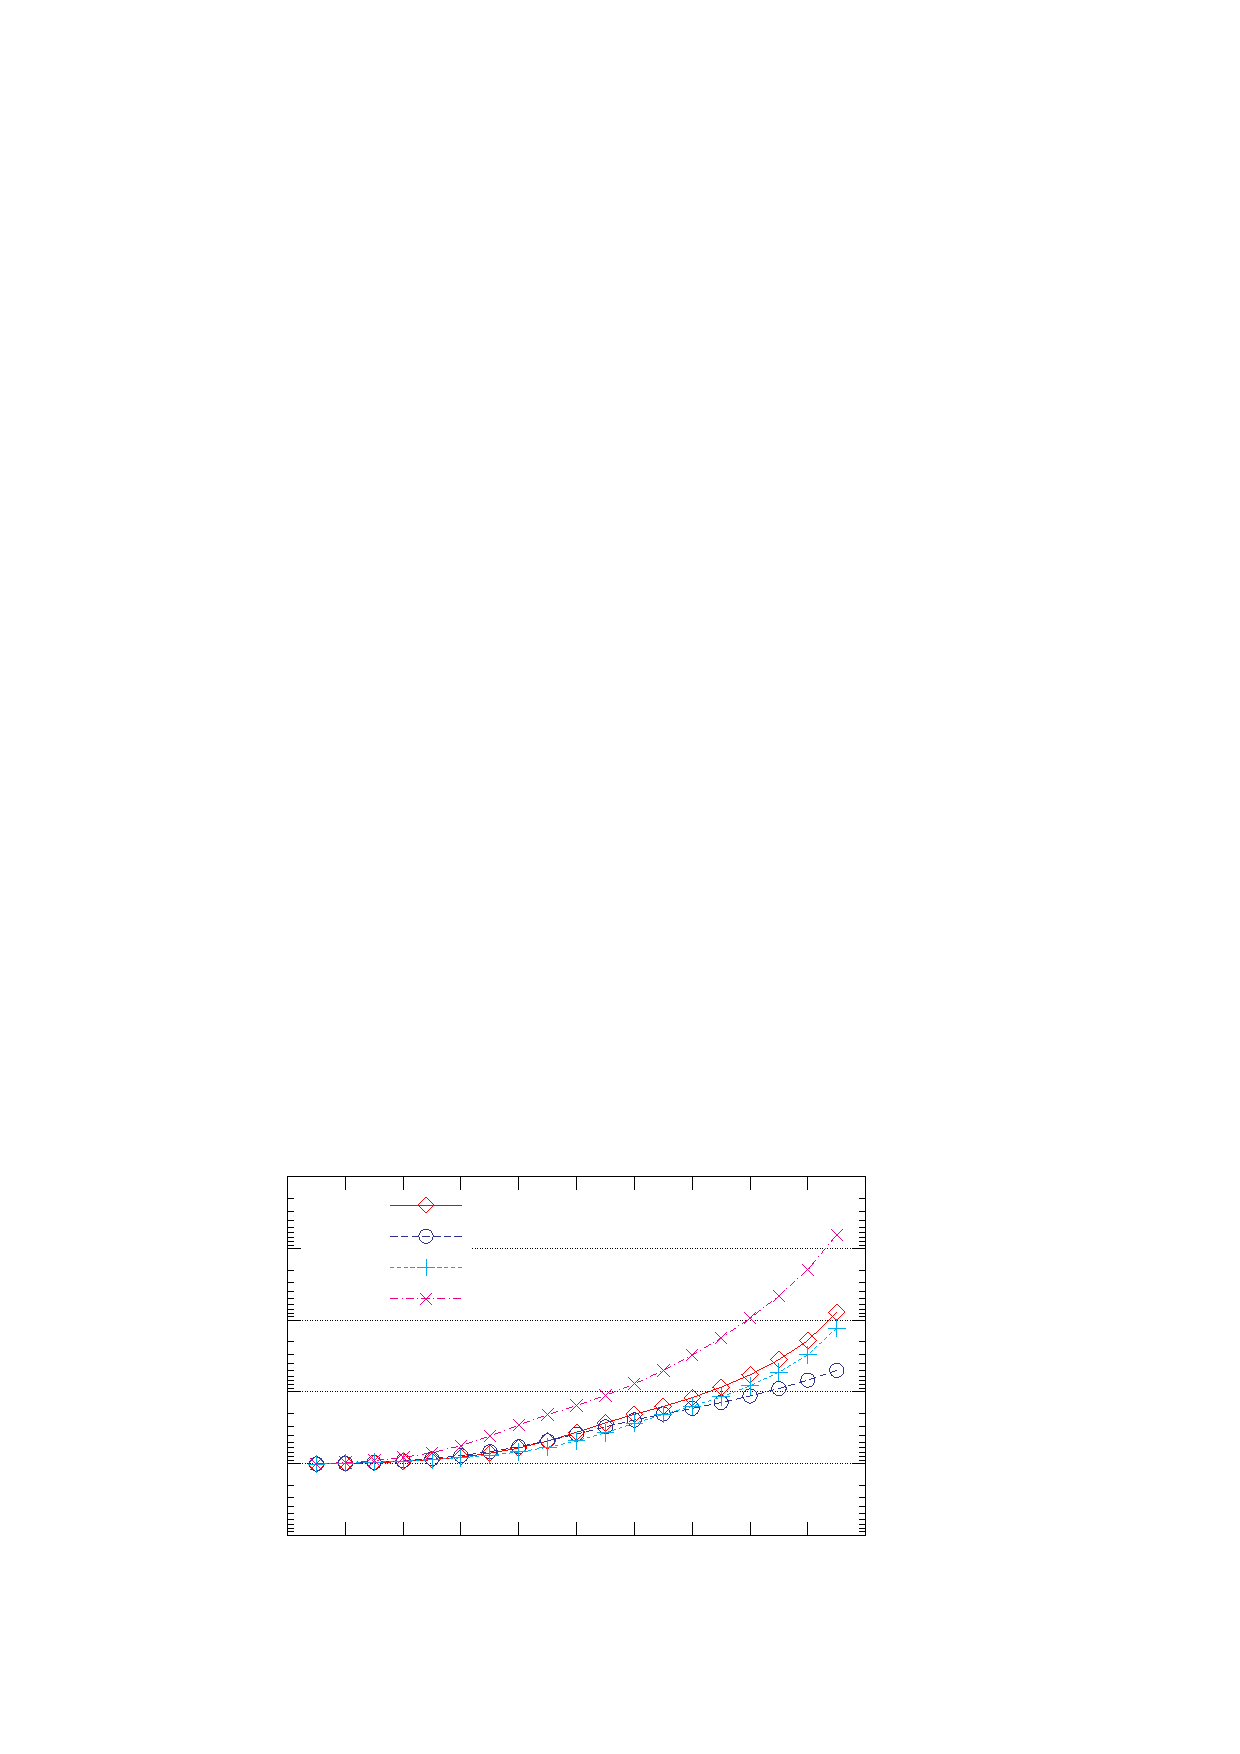
\includegraphics{Graphiques/compare_sampl_19}%
\end{picture}%
\begingroup
\setlength{\unitlength}{0.0200bp}%
\begin{picture}(18000,10800)(0,0)%
\put(3025,10250){\makebox(0,0)[r]{\strut{} 10}}%
\put(3025,8530){\makebox(0,0)[r]{\strut{} 100}}%
\put(3025,6810){\makebox(0,0)[r]{\strut{} 1000}}%
\put(3025,5090){\makebox(0,0)[r]{\strut{} 10000}}%
\put(3025,3370){\makebox(0,0)[r]{\strut{} 100000}}%
\put(3025,1650){\makebox(0,0)[r]{\strut{} 1e+06}}%
\put(3300,1100){\makebox(0,0){\strut{} 0}}%
\put(4688,1100){\makebox(0,0){\strut{} 2}}%
\put(6075,1100){\makebox(0,0){\strut{} 4}}%
\put(7463,1100){\makebox(0,0){\strut{} 6}}%
\put(8850,1100){\makebox(0,0){\strut{} 8}}%
\put(10238,1100){\makebox(0,0){\strut{} 10}}%
\put(11625,1100){\makebox(0,0){\strut{} 12}}%
\put(13013,1100){\makebox(0,0){\strut{} 14}}%
\put(14400,1100){\makebox(0,0){\strut{} 16}}%
\put(15788,1100){\makebox(0,0){\strut{} 18}}%
\put(17175,1100){\makebox(0,0){\strut{} 20}}%
\put(550,5950){\rotatebox{90}{\makebox(0,0){\strut{}\shortstack{pression
        \\ (Pa)}}}}%
\put(10237,275){\makebox(0,0){\strut{}indice}}%
\put(5500,9575){\makebox(0,0)[r]{\strut{}LMD5}}%
\put(5500,8825){\makebox(0,0)[r]{\strut{}param}}%
\put(5500,8075){\makebox(0,0)[r]{\strut{}strato1}}%
\put(5500,7325){\makebox(0,0)[r]{\strut{}strato2}}%
\end{picture}%
\endgroup
\endinput

  \caption[Maillage vertical, échantillonnages de $s$ pour :
  \texttt{llm} = 19]{Maillage vertical.  Comparaison des trois
    échantillonnages de $s$ pour : \texttt{llm} = 19 ; \texttt{h} = 7
    ; \texttt{deltaz} = \np{0,04} ; \texttt{beta} = \np{1,3} ;
    \texttt{k0} = 20 ; \texttt{k1} = \np{1,2}. La pression à la
    surface choisie est de 101325 Pa.}
  \label{fig:compare_sampl_19}
\end{figure}
\begin{figure}[htbp]
  \centering
  \input{Graphiques/compare_sampl_30.tex}
  \caption[Maillage vertical, échantillonnages de $s$ pour :
  \texttt{llm} = 30]{Maillage vertical.  Comparaison des trois
    échantillonnages de $s$ pour : \texttt{llm} = 30 ; \texttt{h} = 7
    ; \texttt{deltaz} = \np{0,04} ; \texttt{beta} = \np{1,3} ;
    \texttt{k0} = 20 ; \texttt{k1} = \np{1,2}. La pression à la
    surface choisie est de 101325 Pa.}
  \label{fig:compare_sampl_30}
\end{figure}
\begin{figure}[htbp]
  \centering
  %GNUPLOT: LaTeX picture with Postscript
\begin{picture}(0,0)%
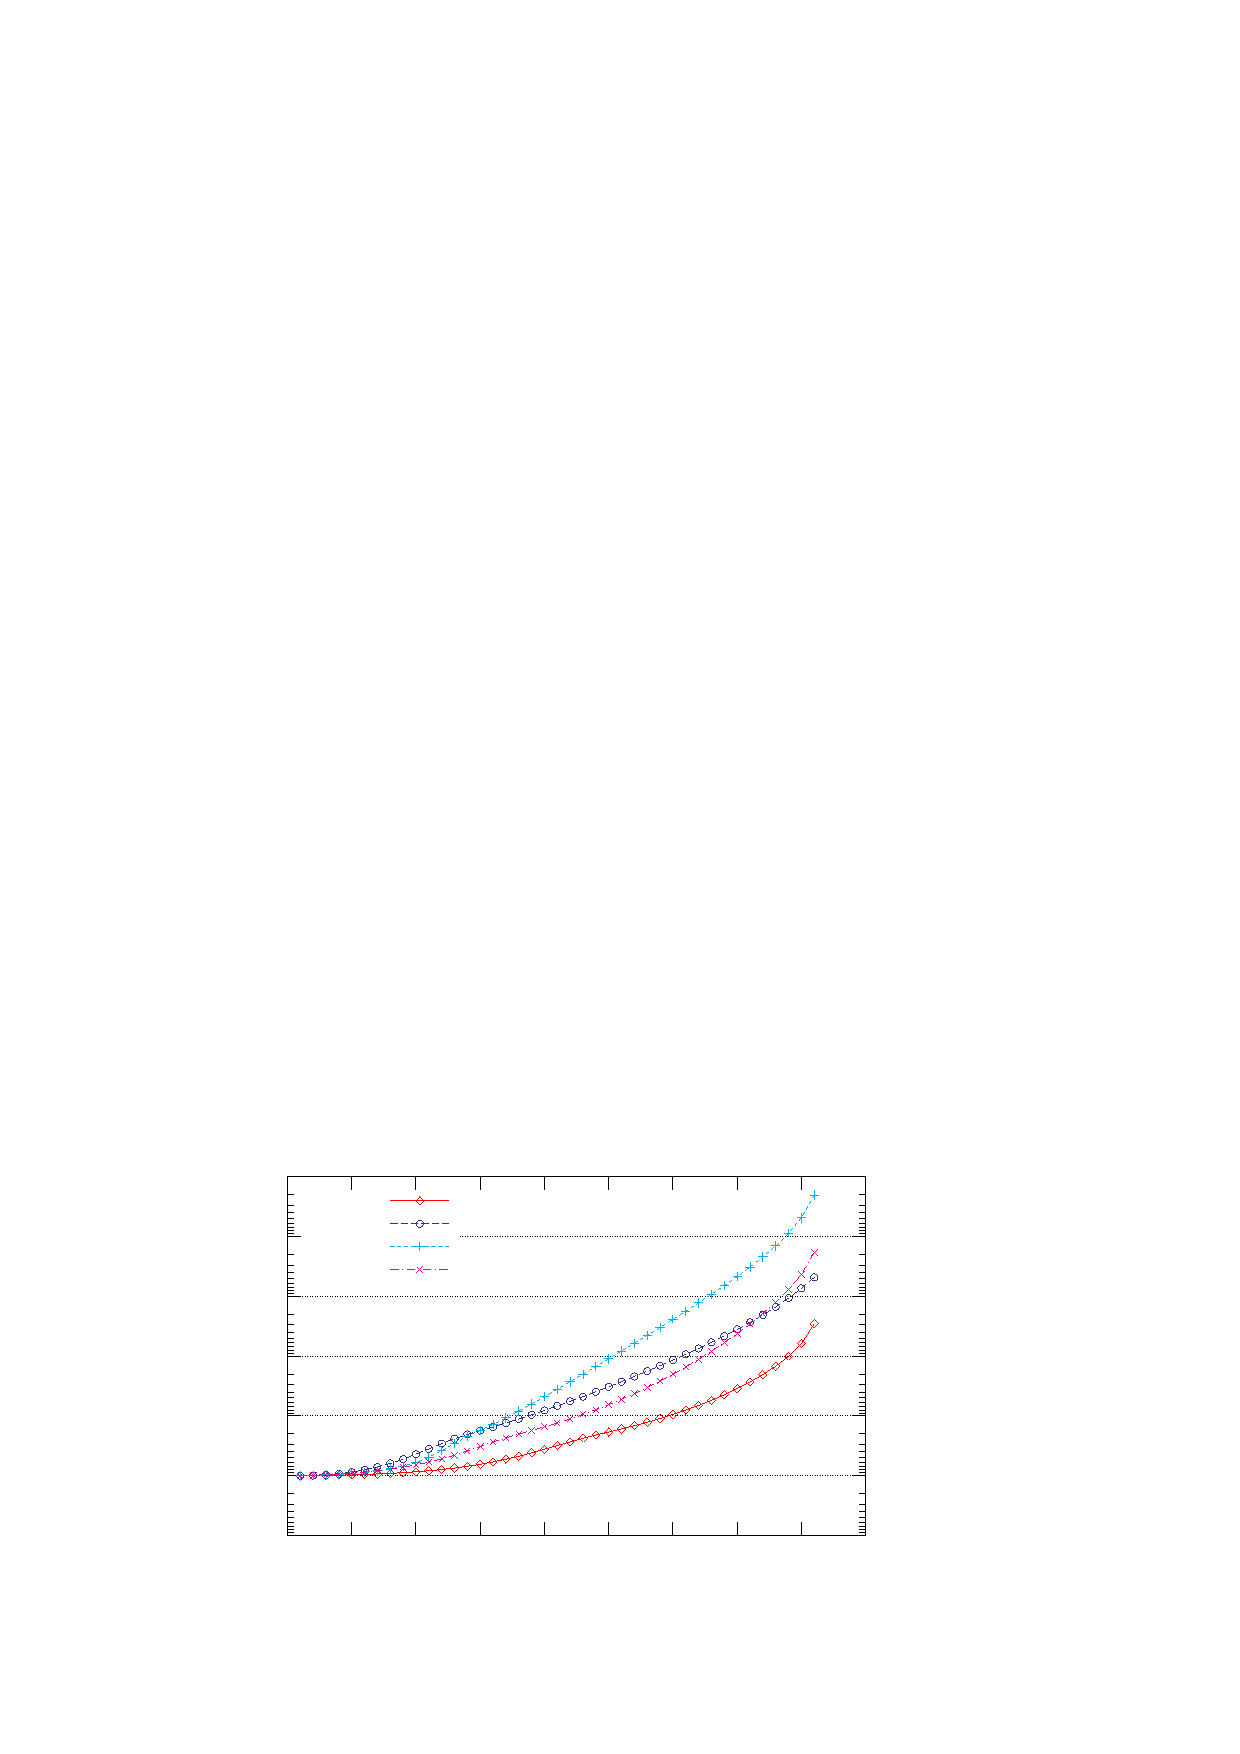
\includegraphics{Graphiques/compare_sampl_41}%
\end{picture}%
\begingroup
\setlength{\unitlength}{0.0200bp}%
\begin{picture}(18000,10800)(0,0)%
\put(3025,10250){\makebox(0,0)[r]{\strut{} 1}}%
\put(3025,8817){\makebox(0,0)[r]{\strut{} 10}}%
\put(3025,7383){\makebox(0,0)[r]{\strut{} 100}}%
\put(3025,5950){\makebox(0,0)[r]{\strut{} 1000}}%
\put(3025,4517){\makebox(0,0)[r]{\strut{} 10000}}%
\put(3025,3083){\makebox(0,0)[r]{\strut{} 100000}}%
\put(3025,1650){\makebox(0,0)[r]{\strut{} 1e+06}}%
\put(3300,1100){\makebox(0,0){\strut{} 0}}%
\put(4842,1100){\makebox(0,0){\strut{} 5}}%
\put(6383,1100){\makebox(0,0){\strut{} 10}}%
\put(7925,1100){\makebox(0,0){\strut{} 15}}%
\put(9467,1100){\makebox(0,0){\strut{} 20}}%
\put(11008,1100){\makebox(0,0){\strut{} 25}}%
\put(12550,1100){\makebox(0,0){\strut{} 30}}%
\put(14092,1100){\makebox(0,0){\strut{} 35}}%
\put(15633,1100){\makebox(0,0){\strut{} 40}}%
\put(17175,1100){\makebox(0,0){\strut{} 45}}%
\put(550,5950){\rotatebox{90}{\makebox(0,0){\strut{}\shortstack{pression \\ (Pa)}}}}%
\put(10237,275){\makebox(0,0){\strut{}indice}}%
\put(5500,9675){\makebox(0,0)[r]{\strut{}LMD5}}%
\put(5500,9125){\makebox(0,0)[r]{\strut{}param}}%
\put(5500,8575){\makebox(0,0)[r]{\strut{}strato1}}%
\put(5500,8025){\makebox(0,0)[r]{\strut{}strato2}}%
\end{picture}%
\endgroup
\endinput

  \caption[Maillage vertical, échantillonnages de $s$ pour :
  \texttt{llm} = 41]{Maillage vertical.  Comparaison des trois
    échantillonnages de $s$ pour : \texttt{llm} = 41 ; \texttt{h} = 7
    ; \texttt{deltaz} = \np{0,04} ; \texttt{beta} = \np{1,3} ;
    \texttt{k0} = 20 ; \texttt{k1} = \np{1,2}. La pression à la
    surface choisie est de 101325 Pa.}
  \label{fig:compare_sampl_41}
\end{figure}
Dans tous les cas, le tableau \verb+s+ doit être strictement
décroissant de 1 à 0.

En supposant $p_s = p_\mathrm{ref}$, notons $\delta$ la différence
d'altitude-pression entre deux niveaux. Pour $l \in \{1, \dots,
\mathtt{llm} - 1\}$ :
\begin{equation*}
  \delta_l := H \ln \frac{p(s_l)}{p(s_{l+1})}
\end{equation*}
Pour \verb+llm+ donné, si on se donne les contraintes :
\begin{align*}
  & p(s_\mathtt{llm}) = \numprint[hPa]{0.1} \\
  & \delta_1 = 60\ \mathrm{m} \\
  & \textrm{pour } l \in \{2, \dots, \mathtt{llm} - 1\},
  \delta_l = \alpha z(s_l) + \delta_1
\end{align*}
alors :
\begin{align*}
  & s_\mathtt{llm} \approx \numprint{5e-4} \\
  & s_2 \approx \numprint{0,9943} \\
  & \textrm{pour } l \in \{2, \dots, \mathtt{llm}\},
  p(s_l) / p_\mathrm{ref}
  = \exp\left(- \frac{\delta_1}{H} \frac{(1 + \alpha)^{l - 1} - 1}{\alpha}\right)
\end{align*}
L'application de cette formule à $l = \mathtt{llm}$ permet d'obtenir
$\alpha$, par exemple par la méthode du point fixe :
\begin{equation*}
  \alpha
  =
  \left[
    \alpha \frac{H}{\delta_1}
    \left(\ln \frac{p_\mathrm{ref}}{p(s_\mathtt{llm})}\right) + 1
  \right]
  ^{\frac{1}{\mathtt{llm} - 1}}
  - 1
\end{equation*}
Pour $p_\mathrm{ref} = \numprint[hPa]{1013.25}$ et $\mathtt{llm} =
39$, on obtient :
\begin{equation*}
  \alpha \approx \numprint{0.1416}
\end{equation*}
Il reste à déduire $s_l$ de $p(s_l)$. La méthode du point fixe pour
trouver $s_l$ peut ne marcher ni dans un sens ni dans l'autre pour un
point au voisinage de $s = \numprint{.5}$, lorsque la dérivée de la
fonction à point fixe est proche de 1.

Si, sur une certaine plage d'indice $l \in \{l_1, \dots, \mathtt{llm}
- 1\}$, $\delta_l = \delta$ est constant alors, pour $l \in \{l_1,
\dots, \mathtt{llm}\}$ :
\begin{displaymath}
  p(s_l)
  = p(s_{l_1}) \left[ \frac{p(s_\mathtt{llm})}{p(s_{l_1})} \right]
    ^{\frac{l - l_1}{\mathtt{llm} - l_1}}
\end{displaymath}
et :
\begin{displaymath}
  \delta = \frac{H}{\mathtt{llm} - l_1} \ln \frac{p(s_{l_1})}{p(s_\mathtt{llm})}
\end{displaymath}

\section{La pression en milieu de couche}

Hypothèses :
{\color{green}
\begin{align*}
  & \mathtt{llm} \ge 1 \\
  & \kappa = 2 / 7 \\
  & p_s \ge p_a
\end{align*}
$(s_{l - 1 / 2})_{l \in \{1, \dots, \mathtt{llm} + 1\}}$ est une suite
strictement décroissante de 1 à 0.
\begin{equation*}
  \forall l \in \{1, \dots, \mathtt{llm} + 1\},
  p_{l - 1 / 2} = a(s_{l - 1 / 2}) + b(s_{l - 1 / 2}) p_s
\end{equation*}
$a$ et $b$ sont donnés par les équations (\ref{eq:a}) et (\ref{eq:b}),
avec $p_a = 500$ hPa.}

Dans la procédure \verb+exner_hyb+, nous utilisons la relation :
\begin{displaymath}
  \overline{p \delta_z \Pi}^z = \kappa \Pi \delta_z p
\end{displaymath}
(cf. \href{http://lmdz.lmd.jussieu.fr/utilisateurs/manuel-de-reference-1/developpeurs/notes-techniques/ressources/documentation-du-modele-de-circulation-generale-atmospherique-lmdz}{documentation
  technique de LMDZ}, § 2.3.3). Développons cette équation, écrite au
milieu de la couche $l$, pour $l \in \{2, \dots, \mathtt{llm} - 1\}$ :
\begin{equation}
  \label{eq:exner}
  \frac{1}{2} [(p \delta_z \Pi)_{l-1/2} + (p \delta_z \Pi)_{l+1/2}]
  = \kappa \Pi_l (\delta_z p)_l
\end{equation}
Pour la couche 1 , il faut trouver la valeur convenable de $(p
\delta_z \Pi)_{1/2}$. Admettons que :
\begin{displaymath}
  (\delta_z \Pi)_{1/2} = 2 (\Pi_1 - \Pi_s)
\end{displaymath}
convient, on peut noter :
\begin{equation}
  \label{eq:def_pi0}
  \Pi_0 := 2 \Pi_s - \Pi_1
\end{equation}
Alors l'équation (\ref{eq:exner}) se généralise aux indices $l \in
\{1, \dots, \mathtt{llm} - 1\}$ et se développe en :
\begin{equation}
  \label{eq:exner_gl}
  p_{l-1/2} (\Pi_l - \Pi_{l-1}) + p_{l+1/2} (\Pi_{l+1} - \Pi_l)
  = 2 \kappa \Pi_l (p_{l+1/2} - p_{l-1/2})
\end{equation}
Pour la couche \verb+llm+, en remarquant que $p_{\mathtt{llm}+1/2} =
0$, nous admettons que l'équation suivante convient :
\begin{equation*}
  \frac{1}{2} (p \delta_z \Pi)_{\mathtt{llm}-1/2}
  = \kappa \Pi_\mathtt{llm} (\delta_z p)_\mathtt{llm}
\end{equation*}
Ce qui donne :
\begin{equation}
  \label{eq:pi_llm}
  \Pi_\mathtt{llm} (1 + 2 \kappa) = \Pi_{\mathtt{llm} - 1}
\end{equation}
$(\Pi_l)_{l \in \{0, \dots, \mathrm{llm}\}}$ est déterminé par la
récurrence \eqref{eq:exner_gl} et par les conditions aux limites
(\ref{eq:def_pi0}) et \eqref{eq:pi_llm}. Supposons :
\begin{equation}
  \label{eq:pi_pos}
  \forall l \in \{0, \dots, \mathtt{llm}\}, \Pi_l \ne 0
\end{equation}
et nous vérifierons l'auto-cohérence de la solution avec cette
hypothèse. Notons, pour $l \in \{1, \dots, \mathtt{llm}\}$ :
\begin{displaymath}
  \beta_{l-1/2} := \Pi_l / \Pi_{l-1}
\end{displaymath}
En divisant l'équation (\ref{eq:exner_gl}) par $\Pi_l$, on obtient,
pour $l \in \{1, \dots, \mathtt{llm} - 1\}$ :
\begin{equation}
  \label{eq:beta_nodiv}
  p_{l-1/2} \left( 1 - \frac{1}{\beta_{l-1/2}} \right) + p_{l+1/2} (\beta_{l+1/2} - 1)
  = 2 \kappa (p_{l+1/2} - p_{l-1/2})
\end{equation}
Avec l'équation \eqref{eq:pi_llm} :
\begin{displaymath}
  \beta_{\mathtt{llm}-1/2} = \frac{1}{1 + 2 \kappa}
\end{displaymath}
donc nous pouvons appliquer la récurrence dans le sens
descendant. L'équation \eqref{eq:beta_nodiv} s'écrit encore :
\begin{equation*}
  p_{l-1/2} / \beta_{l-1/2}
  = (1 + 2 \kappa) (p_{l-1/2} - p_{l+1/2}) + \beta_{l+1/2} p_{l+1/2}
\end{equation*}
Ainsi, si $\beta_{l+1/2} > 0$ alors $\beta_{l-1/2} > 0$ et le membre
de droite ci-dessus est strictement positif. Donc, par récurrence :
\begin{equation*}
  {\color{red}
    \forall l \in \{1, \dots, \mathtt{llm}\}, \beta_{l - 1 / 2} > 0
  }
\end{equation*}
et nous pouvons écrire, pour $l \in \{1, \dots, \mathtt{llm} - 1\}$ :
\begin{align}
  \notag
  \beta_{l-1/2}
  & =
  \frac{p_{l-1/2}}
  {(1 + 2 \kappa) (p_{l-1/2} - p_{l+1/2}) + \beta_{l+1/2} p_{l+1/2}} \\
  \label{eq:beta}
  & =
  \frac{p_{l-1/2}}{(1 + 2 \kappa) p_{l-1/2} + (\beta_{l+1/2} - 1 - 2 \kappa) p_{l+1/2}}
\end{align}
Nous obtenons $\beta_{\mathtt{llm}-3/2}, \dots, \beta_{1/2}$. Par
ailleurs, par définition de $\beta_{1/2}$ et $\Pi_0$ :
\begin{equation}
  \label{eq:pi1}
  \Pi_1 = \frac{2 \beta_{1/2}}{\beta_{1/2} + 1} \Pi_s
\end{equation}
On peut éventuellement développer $\beta_{1/2}$ en fonction de $\beta_{3/2}$
(équation (\ref{eq:beta})) pour obtenir une expression de $\Pi_1$ en
fonction de $\beta_{3/2}$ et $\Pi_s$ :
\begin{displaymath}
  \Pi_1
  =
  \frac{p_s}
  {p_s(1 + \kappa) + \frac{1}{2}(\beta_{3/2} - 1 - 2 \kappa) p_{3/2}} 
  \Pi_s
\end{displaymath}
D'où $\Pi_2, \dots, \Pi_\mathtt{llm}$ par récurrence. La suite
$(s_{l-1/2})_{l \in \{1, \dots, \mathtt{llm} + 1\}}$
étant donnée, les valeurs de $(p_{l-1/2})$, de $(\Pi_l)$ et de :
\begin{displaymath}
  p_l = p_\mathrm{ref} (\Pi_l / c_p)^{1 / \kappa}
\end{displaymath}
ne dépendent que de $p_s$.

Les valeurs obtenues de $\Pi_l$ sont-elles bien strictement positives
? L'équation \eqref{eq:pi1} impose $0 < \Pi_1 < 2 \Pi_s$, donc $\Pi_0
> 0$. Et, par récurrence :
\begin{equation*}
  {\color{red}
    \forall l \in \{0, \dots, \mathtt{llm}\}, \Pi_l > 0
  }
\end{equation*}
Nous avons bien l'auto-cohérence avec l'hypothèse \eqref{eq:pi_pos}.

Les valeurs obtenues de $\Pi_l$ sont-elles par construction
strictement décroissantes ? On a :
\begin{equation}
  {\color{red}
    \label{eq:betalow}
    \forall l \in \{1, \dots, \mathtt{llm} - 1\},
    \beta_{l-1/2} < 1
    \Leftrightarrow
    \frac{p_{l-1/2} - p_{l+1/2}}{p_{l+1/2}} > \frac{1 - \beta_{l+1/2}}{2 \kappa}
  }
\end{equation}
C'est-à-dire que les pressions aux demi-niveaux doivent être
suffisamment écartées. En particulier, si llm $\ge 2$ :
\begin{equation}
  \beta_{\mathtt{llm} - 3/2} < 1
  \Leftrightarrow
  p_{\mathtt{llm} - 3/2} > \frac{2 (1 + \kappa)}{1 + 2 \kappa} p_{\mathtt{llm} - 1/2}
  \label{eq:beta_llm32}
\end{equation}
Si llm = 1 alors :
\begin{equation*}
    \beta_{1/2} = \frac{1}{1 + 2 \kappa} < 1
\end{equation*}
donc $(\Pi_l)$ est bien strictement décroissante. Si llm $\ge 2$, les
degrés de liberté dans la construction des suites $(p_{l-1/2})$,
$(\Pi_l)$ et $(p_l)$ sont : $s_{3/2}, \dots, s_{\mathtt{llm}-1/2}$
($\mathtt{llm} - 1$ valeurs) et $p_s$. Si llm $\ge 3$, pour $l \in
\{2, \dots, \mathtt{llm} - 1\}$, $\beta_{l+1/2}$ est déterminé par
$(s_{l'-1/2})_{l' \ge l + 1}$ et $p_s$, $\beta_{l+1/2}$ ne dépend pas
de $s_{l-1/2}$. Tandis que $p_{l-1/2}$ est déterminé par $s_{l-1/2}$
et $p_s$. Les $\beta_{l-1/2}$ ne sont donc pas par construction
strictement inférieurs à 1. On peut exhiber un contre-exemple :
\begin{align*}
  & \mathtt{llm} = 3 \\
  & p_s = \np[hPa]{1013.25}
\end{align*}
La condition (\ref{eq:beta_llm32}) avec $p_{5/2} = 150$ hPa s'écrit :
\begin{displaymath}
  \beta_{3/2} < 1
  \Leftrightarrow p_{3/2} > \np[hPa]{245}
\end{displaymath}
Cf. figure (\ref{fig:counter_ex}).
\begin{figure}[htbp]
  \centering
  \includegraphics{counter_ex}
  \caption[Distribution verticale mal choisie]{Distribution verticale
    mal choisie. Les niveaux pleins sont en rouge. Une valeur de
    $\beta$ est supérieure à 1 et les pressions aux niveaux pleins ne
    sont pas intercalées entre les presssions aux demi-niveaux.}
  \label{fig:counter_ex}
\end{figure}

Les pressions $p_l$ correspondant aux $\Pi_l$ sont-elles bien
intercalées entre les pressions aux demi-niveaux ? Avec les équations
(\ref{eq:pi1}) et (\ref{eq:def_pi0}):
\begin{displaymath}
  {\color{red}
    \Pi_1 < \Pi_s < \Pi_0 \Leftrightarrow \beta_{1/2} < 1
  }
\end{displaymath}
Donc pour llm = 1, les pressions $p_l$ correspondant aux $\Pi_l$ sont
toujours bien intercalées entre les pressions aux demi-niveaux. Pour
llm $\ge 2$, la réponse est négative. J'ai constaté que, avec
certaines suites $(s_{l-1/2})$, $\beta_{1/2} \ge 1$. De plus, j'ai
constaté dans certains cas que les pressions $p_l$ correspondant aux
$\Pi_l$, à d'autres couches que la couche 1, ne sont pas intercalées
entre les pressions aux demi-niveaux. Cf. par exemple figure
(\ref{fig:counter_ex}).

On peut se poser une question encore plus précise (c'est-à-dire avec
des hypothèses plus fortes). Pour llm $\ge 2$, pour une distribution
verticale $(s_l)$ donnée, supposons qu'il existe une valeur
particulière de pression à la surface telle que :
\begin{equation}
  \label{eq:hyp_ps0}
  \forall l \in \{1, \dots, \mathtt{llm}\}, p_{l - 1 / 2} > p_l > p_{l + 1 / 2}
\end{equation}
On remarque que cela implique :
\begin{equation*}
  \forall l \in \{1, \dots, \mathtt{llm}\}, \beta_{l - 1 / 2} < 1  
\end{equation*}
A-t-on alors la propriété (\ref{eq:hyp_ps0}) pour toute valeur de
$p_s$ ? La réponse est négative. Exhibons un contre-exemple avec llm =
2. Pour llm = 2 :
\begin{equation*}
    \beta_{3/2} = \frac{1}{1 + 2 \kappa}
\end{equation*}
Avec l'équation (\ref{eq:betalow}) :
\begin{equation*}
  \beta_{1/2} < 1
  \Leftrightarrow p_s > \frac{2 (1 + \kappa)}{1 + 2 \kappa} p_{3/2}
\end{equation*}
Explicitons la dépendance en $p_s$ :
\begin{equation*}
  p_{3/2} = a_{3/2} + b_{3/2} p_s
\end{equation*}
Notons :
\begin{equation*}
  \alpha := \frac{2 (1 + \kappa)}{1 + 2 \kappa} = 18 / 11 > 1
\end{equation*}
On a :
\begin{equation*}
  \beta_{1/2} < 1
  \Leftrightarrow p_s (1 - \alpha b_{3/2}) > \alpha a_{3/2}
\end{equation*}
Une valeur particulière de $s_{3/2}$ intervient :
\begin{equation*}
  b_{3/2} = 1 / \alpha
  \Leftrightarrow s_{3/2} = 1 / \sqrt{1 + \ln \alpha} \approx \np{.82}
\end{equation*}
Si $s_{3/2} \ge 1 / \sqrt{1 + \ln \alpha}$ alors :
\begin{equation*}
  \forall p_s, \beta_{1/2} \ge 1
\end{equation*}
Ce n'est pas le cas qui nous intéresse. Si $s_{3/2} < 1 / \sqrt{1 +
  \ln \alpha}$ alors :
\begin{equation*}
  \beta_{1/2} < 1
  \Leftrightarrow p_s > \frac{\alpha a_{3/2}}{1 - \alpha b_{3/2}}
\end{equation*}
(Remarque : on peut montrer que $\frac{\alpha a_{3/2}}{1 - \alpha
  b_{3/2}}$ est une fonction strictement croissante de $s_{3/2}$ pour
$s_{3/2} \in [0, 1 / \sqrt{1 + \ln \alpha}[$.) Nous avons donc notre
contre-exemple. On peut prendre par exemple $s_{3/2} = \np{.7}$, ce qui
donne :
\begin{equation*}
  \frac{\alpha a_{3/2}}{1 - \alpha b_{3/2}} \approx \np[hPa]{672}
\end{equation*}
Cf. figure (\ref{fig:test_disvert}).
\begin{figure}[htbp]
  \centering
  \includegraphics[width=\textwidth]{test_disvert}
  \caption[Ordre des pressions dépendant de $p_s$]{Pour une même suite
    $(s_l)$, l'ordre des pressions peut être correct pour une valeur
    de $p_s$ et incorrect pour une autre valeur de $p_s$. Ici, llm = 2
    et $s_{3/2} = \np{.7}$. Les niveaux pleins sont en rouge. Les
    valeurs sont les pressions en hPa, dans deux colonnes.}
  \label{fig:test_disvert}
\end{figure}
$\Box$

Si la pression $p_1$ correspondant à $\Pi_1$ est supérieure à $p_s$
alors \verb+zgeop(i, 1)+ dans la procédure \verb+coefkz+ est négatif,
d'où un argument du logarithme qui peut être négatif dans le calcul de
\verb+zcdn+, dans la procédure \verb+clcdrag+.

Pour la distribution verticale de CMIP5 (39 couches), je
constate :
\begin{equation*}
  \forall l \ge 21,
  \max_{\lambda, \phi} p_l / \min_{\lambda, \phi} p_l - 1 = \np{0.0056174993515}
\end{equation*}
(exactement constant), correspondant à des pressions inférieures à 110
hPa environ. De plus, les valeurs de presnivs sont assez différentes,
avec des écarts jusqu'à 15 \%, au somment de l'atmosphère. De même,
pour la distribution verticale de CMIP6 (79 couches), les interfaces
sont des niveaux de pression pour $l \ge 45$, $p \le 130$ hPa mais,
pour les pressions inférieures à 160 hPa :
\begin{equation*}
  \max_{\lambda, \phi} p_l / \min_{\lambda, \phi} p_l - 1
  \approx \np{2e-3}
\end{equation*}
jusqu'au somment, pratiquement constant. Les écarts entre presnivs et
pres dans les 10 niveaux supérieurs sont de l'ordre de 1 \% à 10 \%.

\section{Cas \texttt{tropo}}

Pour $l \in \{1, \dots,
\mathtt{llm}\}$, posons :
\begin{displaymath}
  x_l = \frac{\pi (l - 1/2)}{\mathtt{llm} + 1}
\end{displaymath}
Pour $x \in \mathbb{R}$, posons :
\begin{displaymath}
  f(x) = 1 + 7 \sin^2 x
\end{displaymath}
$f$ est périodique de période $\pi$. Cf. figure (\ref{fig:f_x}).
\begin{figure}[htbp]
  \centering
  %GNUPLOT: LaTeX picture with Postscript
\begin{picture}(0,0)%
\includegraphics{Graphiques/f_x}%
\end{picture}%
\begingroup
\setlength{\unitlength}{0.0200bp}%
\begin{picture}(18000,10800)(0,0)%
\put(1650,1650){\makebox(0,0)[r]{\strut{} 1}}%
\put(1650,2879){\makebox(0,0)[r]{\strut{} 2}}%
\put(1650,4107){\makebox(0,0)[r]{\strut{} 3}}%
\put(1650,5336){\makebox(0,0)[r]{\strut{} 4}}%
\put(1650,6564){\makebox(0,0)[r]{\strut{} 5}}%
\put(1650,7793){\makebox(0,0)[r]{\strut{} 6}}%
\put(1650,9021){\makebox(0,0)[r]{\strut{} 7}}%
\put(1650,10250){\makebox(0,0)[r]{\strut{} 8}}%
\put(1925,1100){\makebox(0,0){\strut{} 0}}%
\put(4352,1100){\makebox(0,0){\strut{} 0.5}}%
\put(6779,1100){\makebox(0,0){\strut{} 1}}%
\put(9206,1100){\makebox(0,0){\strut{} 1.5}}%
\put(11633,1100){\makebox(0,0){\strut{} 2}}%
\put(14061,1100){\makebox(0,0){\strut{} 2.5}}%
\put(16488,1100){\makebox(0,0){\strut{} 3}}%
\put(550,5950){\rotatebox{90}{\makebox(0,0){\strut{}f(x)}}}%
\put(9550,275){\makebox(0,0){\strut{}x}}%
\end{picture}%
\endgroup
\endinput

  \caption{Maillage vertical, fonction utilisée dans le cas
    \texttt{tropo}.}
  \label{fig:f_x}
\end{figure}
$(x_l)$ est un échantillonnage de $[0, \pi]$ d'autant plus fin que
\verb+llm+ est grand :
\begin{align*}
  & \forall l \in \{1, \dots, \mathtt{llm}\}, x_l \in ]0, \pi[ \\
  & \exists \lim_{\mathtt{llm} \to +\infty} x_1 = 0 \\
  & \exists \lim_{\mathtt{llm} \to +\infty} x_\mathtt{llm} = \pi \\
  & x_{l+1} - x_l = \frac{\pi}{\mathtt{llm} + 1}
  \underset{\mathtt{llm} \to + \infty}{\longrightarrow} 0
\end{align*}
Le programme calcule :
\begin{displaymath}
  \mathtt{ds(l)} = \frac{f(x_l)}{\sum_{l'=1}^\mathtt{llm} f(x_{l'})}
\end{displaymath}
puis :
\begin{align*}
  s_l & = \sum_{l' = l}^\mathtt{llm} \mathtt{ds(l)} \\
  & = \frac{\sum_{l' = l}^\mathtt{llm} f(x_{l'})}{\sum_{l'=1}^\mathtt{llm} f(x_{l'})}
\end{align*}
Or :
\begin{displaymath}
  \sum_{l=1}^\mathtt{llm} f(x_{l}) \frac{\pi}{\mathtt{llm} + 1}
  \underset{\mathtt{llm} \to + \infty}{\longrightarrow} \int_0 ^\pi f
\end{displaymath}
Notons :
\begin{displaymath}
  I := \int_0 ^\pi f = 9 \pi / 2
\end{displaymath}
On a donc :
\begin{displaymath}
  \sum_{l=1}^\mathtt{llm} f(x_{l})
  \underset{\mathtt{llm} \to +\infty}{\sim} \frac{I}{\pi} \mathtt{llm}
\end{displaymath}
(L'erreur est de 2 \% environ pour \verb+llm+ = 41.) Le niveau
$s$ le plus petit est 0, le deuxième plus petit est :
\begin{displaymath}
  s(\mathtt{llm}) = \mathtt{ds(llm)}
  \underset{\mathtt{llm} \to +\infty}{\sim} \frac{\pi f(\pi)}{I\ \mathtt{llm}}
\end{displaymath}

Donc :
\begin{displaymath}
  p(s(\mathtt{llm}))
  \underset{\mathtt{llm} \to +\infty}{\sim}
  \frac{\pi f(\pi) p_a}{I\ \mathtt{llm}}
  = \frac{2 p_a}{9\ \mathtt{llm}}
\end{displaymath}
On a :
\begin{align*}
  & \mathtt{llm} = 9 \Rightarrow \mathtt{ap(llm)}
  \approx 3 \cdot 10\ \mathrm{hPa} \\
  & \mathtt{llm} = 19 \Rightarrow \mathtt{ap(llm)} \approx 8\ \mathrm{hPa} \\
  & \mathtt{llm} = 50 \Rightarrow \mathtt{ap(llm)} \approx 2\ \mathrm{hPa}
\end{align*}
Il faudrait prendre \verb+llm+ de l'ordre de $10^3$ pour résoudre la
région décrite par la paramétrisation de la chimie de l'ozone.

\section{Cas \texttt{strato}}

C'est le cas conseillé par François L. pour un domaine incluant la
stratosphère. Ce cas est analogue au cas \verb+tropo+. Seule la
fonction $f$ utilisée change. Pour $x \in \mathbb{R}$, posons :
\begin{displaymath}
  g(x)
  = \frac{1}{2} \left[1 - \tgh\left(\frac{x - \pi / 2}{\pi / 2}\right)\right]
\end{displaymath}
Par rapport à la fonction $\tgh$, $g$ est translatée de $\pi / 2$ vers
la droite, dilatée horizontalement d'un facteur $\pi / 2$, inversée
verticalement, translatée verticalement de 1 et contractée
verticalement d'un facteur 2. Elle décroît donc de 1 à $-1$. La
fonction $f$ utilisée est maintenant :
\begin{displaymath}
  f(x) = (1 + 7 \sin^2 x) g(x)^2
\end{displaymath}
Cf. figure (\ref{fig:strato}).
\begin{figure}[htbp]
  \centering
  \input{Graphiques/strato.tex}
  \caption[Maillage vertical, cas \texttt{strato}]{Maillage vertical,
    cas \texttt{strato}. $f(\pi) \approx \np{0,014}$.}
  \label{fig:strato}
\end{figure}
On a :
\begin{displaymath}
  I := \int_0 ^\pi f \approx \np{4,02}
\end{displaymath}
donc :
\begin{displaymath}
  p(s(\mathtt{llm}))
  \underset{\mathtt{llm} \to +\infty}{\sim}
  \frac{\pi f(\pi) p_a}{I\ \mathtt{llm}}
  = \frac{\np{0,011} p_a}{\mathtt{llm}}
\end{displaymath}
Cf. \href{file:///user/guez/Documents/Around_LMDZ/strato_50.odg}{niveaux
  de pressions pour \texttt{llm} = 50}.

Avec l'altitude-pression :
\begin{displaymath}
  z = H \ln \frac{p_s}{p}
\end{displaymath}
on peut avoir une idée de l'épaisseur des couches. Cf.
\href{file:///../delta_z.pdf}{figure dans le cas \texttt{llm} = 50}. Il
y a un maximum local vers $z = 7$ km, niveau numéro 17. Expliquons ce
maximum local. Nous avons :
\begin{displaymath}
  \delta z \approx \frac{\ud z}{\ud s} \delta s
\end{displaymath}
Au niveau 17, $s \approx \np{0,6}$. La figure (\ref{fig:dz_ds})
montre un minimum local de $\frac{\ud z}{\ud s}$ en $s \approx
\np{0,6}$. Par ailleurs, à une constante multiplicative négative
près, $\delta s$ est donné par la fonction $f$. Or, pour $l = 17$ et
\verb+llm+ = 50, $x \approx \np{1,1}$. Nous sommes donc à un
minimum de $\delta s$. $\Box$

\end{document}
